\documentclass{article}
\usepackage{amsmath}
\usepackage{amssymb}
\usepackage{graphicx}
\usepackage{hyperref}
\usepackage[version=4]{mhchem}

\title{Example 20}
\date{}

\begin{document}
\maketitle

(1994 Canadian Mathematical Olympiad) Let \(A B C\) be an acute angled triangle. Let \(A D\) be the altitude on \(B C\), and let \(H\) be any interior point on \(A D\). Lines \(B H\) and \(C H\), when extended, intersect \(A C\) and \(A B\) at \(E\) and \(F\), respectively. Prove that \(\angle E D H=\angle F D H\).\\
\centering
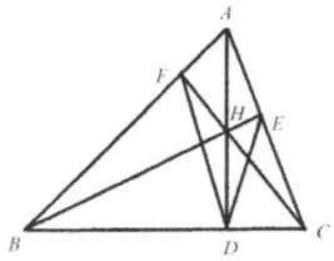
\includegraphics[width=\textwidth]{images/problem_image_1.jpg}

Solution:
Draw \(E P \perp B C\) to meet \(C F\) at \(M\) and \(B C\) at \(P\).\\
Draw \(F Q \perp B C\) to meet \(B E\) at \(N\) and \(B C\) at \(Q\).\\
\(E P / / A D / / F Q\)

\[
\frac{F N}{F Q}=\frac{A H}{A D}=\frac{E M}{E P}, \text { or } \frac{F N}{E M}=\frac{F Q}{E P}
\]

We see that \(\triangle E M H \sim \triangle N H F, D P, D Q\) are the heights of \(\triangle E M H\) and \(\triangle N H F\), respectively. So we have\\
\centering
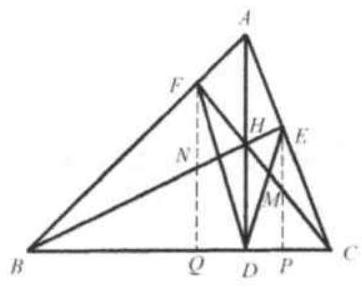
\includegraphics[width=\textwidth]{images/reasoning_image_1.jpg}

\[
\frac{F N}{E M}=\frac{D Q}{D P}
\]

From (1) and (2), \(\frac{F Q}{E P}=\frac{D Q}{D P}\). Thus \(\triangle F Q D \sim \triangle E P D\), and \(\angle F D Q=\angle E D P\).\\
So \(\angle E D H=\angle F D H\).


\end{document}
